\documentclass[11pt]{article}

\usepackage{setspace}
\usepackage{inputenc}
\usepackage[margin=1in]{geometry}
\usepackage{subfig}
\usepackage{graphicx}
\usepackage{multirow}
\usepackage{array}
\usepackage[title]{appendix}
\newcolumntype{M}[1]{>{\centering\arraybackslash}m{#1}}


\title{%
Model Comparison for Bird Species Identification\\
  \large ISyE 6740 - Spring 2022 Project Report}
\author{Team Members: Joe Laniado (GTID: 903233267)}


\begin{document}
\begin{singlespace}
\begin{titlepage}
\maketitle

\end{titlepage}
\tableofcontents
\clearpage

\section{Problem Statement}
Ever since computers were created, we have been trying to find ways for them to automate difficult tasks and make our lives easier. Things like finding the shortest path between two places, drawing a three dimensional floor plan for a new skyscraper, or even doing complex mathematical calculations in seconds; have become as trivial as just opening your phone or laptop and asking a question. One of such questions that came up during the late 1960s was: If we give eyes to a computer, would it know what it was looking at? 
Of course the answer was no, but then the goal became to find a way to teach it how to do it. This was the birth of the scientific field of computer vision. This discipline deals with analyzing, processing, and uderstanding visual data in a way which allows a computer to see an image or video, and be able to extract information and make conclusions from it. Using X-ray scans for automatic diagnosis of lung diseases in patients, or collecting quantitive information about the traffic flow of a city using only a camera; are some notable applications of this that are currently in use. \\

After pondering the applications of such computational advancements while doing some bird watching near my home I started to wonder if there could be a way to use computer vision to simplify the process of identifying our feathered friends. I wanted to develop an image classification model that by training it using labeled pictures of different types of birds; if given new input, it could correctly identify which species the new birds belonged to in a quick and efficient way. This process would save me so much time of manual classification of hundreds of pictures of birds in my camera that I just haven't had the time to sit down and check. Fellow local scientists and bird watching enthusiasts have also expressed excitement over the creation of such a model. Furthermore, out in the field spotting a bird could last only a couple of seconds before it flies away, so any time saved on identifiying the species could be used on monitoring other behaviours or collecting scientific information about such a sight. For this a real time video classifier could be used in order to detect and classify the bird before it flies away, although such a project would be a little more advanced than a simple image classifier. \\

Using the different algorithms learned in class, there is a number of ways to approach the development of our bird species identifier. By means of dimensionality reduction, density estimation, traditional classification algorithms, and deep learning; we will build and compare different image classification models until we find the most accurate and efficient approach to correctly identify the species of each bird. We will evaluate each model with a number of performance variables and analyze their behaviour for this specific classification task. Finally, the best model will be selected and further scalability and functionality implementations will be discussed. \\

\section{Data Source}

The original dataset consists of pictures from more than 400 different species of birds. This includes 58388 training images, 2000 test images, and 2000 validation images. When it comes to the images themselves; each picture is a 224 x 224 x 3 RGB image in jpg format, and contains only one bird per image. The bird usually takes more than 50\% of the pixels in the image making it convenient for training purposes. All images were collected from the BIRDS 400 dataset found at https://www.kaggle.com/gpiosenka/100-bird-species. One important thing to note is that 85\% of the images are from the male of the species and only 15\% are female, this is due to the male having more colors and features that make them more easily recognizible. Due to the big size of the data 7 different species were selected in order to save time and reduce complexity when implementing each approach for our classifier. More species could be added whenever an optimal classifier is selected. Figure 1 shows the selected species that will be used to prototype and test each classifier:\\

\begin{figure}[h]
    \centering
    
    \subfloat[Black Broadbill]{
        \label{ref_lael1}
        \includegraphics[width=0.2\textwidth]{data/birds/train/1BLACK YELLOW BROADBILL/001.JPG}
    }
    \subfloat[Flamingo]{
        \label{ref_lbel4}
        \includegraphics[width=0.2\textwidth]{data/birds/train/2FLAMINGO/011.JPG}
    } 
    \subfloat[Bald Eagle]{
        \label{ref_label1}
        \includegraphics[width=0.2\textwidth]{data/birds/train/3BALD EAGLE/019.JPG}
    }
    \subfloat[Annas Hummingbird]{
        \label{ref_label2}
        \includegraphics[width=0.2\textwidth]{data/birds/train/4ANNAS HUMMINGBIRD/006.JPG}
    }
    \subfloat[Scarlet Macaw]{
        \label{ref_label3}
        \includegraphics[width=0.2\textwidth]{data/birds/train/5SCARLET MACAW/016.JPG}
    }\\
    \subfloat[Ground Hornbill]{
        \label{ref_label3}
        \includegraphics[width=0.2\textwidth]{data/birds/train/9ABYSSINIAN GROUND HORNBILL/007.JPG}
    }
     \subfloat[Touchan]{
        \label{ref_label4}
        \includegraphics[width=0.2\textwidth]{data/birds/train/6TOUCHAN/013.JPG}
    }
    
    
    \caption{Selected Species}
    \label{selected species}
\end{figure}

The following distribution of pictures applies for each species selected:
\begin{itemize}
\item Training: 120
\item Validation: 5
\item Testing: 5
\end{itemize}

The total distribution ends up being 840 for training, 35 for validation, and 35 for testing. 120 images per species may not be enough to prevent overfitting in our model leading to poor generalization results. This will need to be addressed in the methodology.  \\

\section{Methodology}
\subsection{Data Pre-Processing}

For efficiency purposes each RGB image was resized to be 64x64x3 pixels, they were then vectorized into the form 1x12,288 and collected into three different matrices for each category: training, validation, and testing. Each row of this matrices represents a singular picture, and each column the pixel values. Each matrix was labeled depending on the species it came from and assembled into dictionaries, where the key-value pair was the species name and the specific matrix respectively. It is important to note that the images were not transformed into grayscale due to color being such an important feature when classifying birds. Furthermore, the disparity between male and female specimens was determined that while it would probably introduce some level of error into our model, in this case it would be used to test the generalization to different cases when performing the classification. At least until more data is available.\\

One area of concern was that due to the high variability between picture design, 120 images per species might not be good enough to capture the complexity of poses and states that the bird could present. This would cause our model to overfit and not generalize well when testing new kinds of pictures. To solve this problem, slight data augmention was implemented to increase the number of samples we had. In order to maintain model efficiency while testing different approches, only rotation and flipping were implemented in order to multiply our training images from 840 samples to 5,880, or 840 samples per species. Operations like cropping, contrast, translation, and more could be used if more training data is needed for future applications. \\

\subsection{Dimensionality Reduction}
The first approach implements a dimensionality reduction technique to find the most representative combination of features for each species and then compare it to a test picture to make a classification. We start by defining our training images as a $M$x$N$ matrix X, where $M$ represents the number of samples and $N$ the number of pixels as stated in the pre-processing step. To better understand the math behind this technique, it is important to know the following concepts: \\

\begin{enumerate}
\item The theorem for singular value decomposition states that for a rectangular matrix A: $ A_{MxN} = U_{MxM}S_{MxN}V_{NxN}$. Where U and V are orthonormal, $U$ represents the left singular vectors, $S$ the singular values, and $V^T$ the right singular vectors of our matrix.
\item We also know that for a NxN matrix W, there exists an eigenvector u if:
$$ Wu = \lambda u $$ 
Where $\lambda$ is a scalar that represents the eigenvalue and $u$ the eigenvalue of W. \\
\end{enumerate}

The basic Idea of this approach is that for each species of bird, we will find the first $K$ principal components that encompasses it's most representative features by means of singular value decomposition. Using this ``Eigenbirds'' we will then find the projection residual between each test image and all the selected $K$ principal components for each species. The test image will be labeled as the type of bird that produces the lowest residual in this equation. \\

\begin{enumerate}
\item The first step to perform this eigendecomposition is to center our data. To do this we find the mean image $\mu$ for our training data $X$ and use it to center all of our training images by substracting this value from each row. This is necessary in order to better perform the change of basis into the eigenspace. We will also divide all the data by 255 to scale for computational efficiency. The following operation can be shown as:
$$ \mu = \frac{1}{m}\sum_{i=0}^{m}X_i $$
$$ X = (X-\mu)/255 $$

If we reshape the mean to it's original dimensions and plot it as an image for each species we get the following (Figure 2): \\

\begin{figure}[h]
    \centering
    
    \subfloat[Black Broadbill]{
        \label{ref_labe1}
        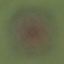
\includegraphics[width=0.2\textwidth]{plots/meanbird-BLA.jpg}
    }
    \subfloat[Flamingo]{
        \label{ref_labe4}
        
\includegraphics[width=0.2\textwidth]{plots/meanbird-FLA.jpg}
    } 
    \subfloat[Bald Eagle]{
        \label{ref_labe1}
        
\includegraphics[width=0.2\textwidth]{plots/meanbird-BAL.jpg}
    } 
    \subfloat[Annas Hummingbird]{
        \label{ref_labe2}
        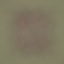
\includegraphics[width=0.2\textwidth]{plots/meanbird-ANN.jpg}
    }
    \subfloat[Scarlet Macaw]{
        \label{ref_labe3}
        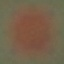
\includegraphics[width=0.2\textwidth]{plots/meanbird-SCA.jpg}
    }
    
    \caption{Mean Image for each species training pictures.}
\end{figure}

\item The eigendecomposition of our centered data can be performed in one of two ways, the first is by finding the eigenvectors, and values of the covariance matrix of X which can be defined as: $ C = XX^T $. this symetric matrix can be diagonalized in the form: 
$$ C = ULU^T$$ 
Where U is a matrix of eigenvectors and L is a diagonal matrix with eigenvalues $\lambda_i$. The second method that can be used is to apply the SVD theorem directly into the transpose of our rectangular matrix X: $X^T = USV^T$, where $U$ would represent our eigenvectors and $S$ the square root of the eigenvalues. The relationship of both approaches can be confirmed by plugging the result of the SVD into our covariance matrix:
$$ X^T = USV^T  \rightarrow C = USV^TVSU^T = US^2U^T$$
Giving us the diagonalized matrix that we got at the beginning of this step. If we were to grab the first principal component for the first 5 species and visualize it, we would get the following result (figure 3):

\begin{figure}[h]
    \centering
    
    \subfloat[Black Broadbill]{
        \label{ref_labe1}
        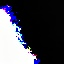
\includegraphics[width=0.2\textwidth]{plots/eigenbird-BLA.jpg}
    }
    \subfloat[Flamingo]{
        \label{ref_labe4}
        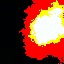
\includegraphics[width=0.2\textwidth]{plots/eigenbird-FLA.jpg}
    } 
    \subfloat[Bald Eagle]{
        \label{ref_labe1}
        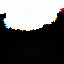
\includegraphics[width=0.2\textwidth]{plots/eigenbird-BAL.jpg}
    }
    \subfloat[Annas Hummingbird]{
        \label{ref_labe2}
        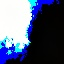
\includegraphics[width=0.2\textwidth]{plots/eigenbird-ANN.jpg}
    }
    \subfloat[Scarlet Macaw]{
        \label{ref_labe3}
        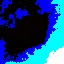
\includegraphics[width=0.2\textwidth]{plots/eigenbird-SCA.jpg}
    }
    
    \caption{1st principal component for the first 5 species visualized as a picture.}
\end{figure} 

This principal components represent the most important features for each species of birds and will be used to perform our classification, due to only being the first of K components each one of this pictures represents a very small amount of variance, only very fine details and combinations of color values con be seen in each image. it may appear random but when put together with the rest of principal components we get a pretty good estimate of the most significant features for each species.

\item Finally, for each test image $y_i$ and each species $j$; we find the projection residual by:

$$ Z_i = (y_i - \mu_j )/255$$
$$ Projection Residual = || Z_i - U_jU_j^TZ_i ||^2_2 $$ 

Where $Z_i$ is the centered vector for image $y_i$ using the mean $\mu_j$ of species $j$ and $U_j$ represents the first K principal components for species $j$. After looping through each test image-species combination, the result will be a MxK matrix where each row represents one of $M$ test images and each column the residual when compared to all $K$ species. All is left to do is to find the minimum residual in each row, and that will give us the predicted species for each test image.
\end{enumerate}

The question remains on choosing how many principal components $K$ to use when calculating our projection residual. This can be addresed by plotting the amount of variance that each principal component explains in the data and choosing a cutoff point where the amount of explained variance becomes negligible. In this case, after performing SVD for the first 5 species of birds and getting the respective eigenvalues they were plotted with respect to each eigenvector in figure 4 to show the explained variance of each principal components for each species. \\

\begin{figure}[h]
    \centering
    
    \subfloat[Black Broadbill]{
        \label{ref_labe1}
        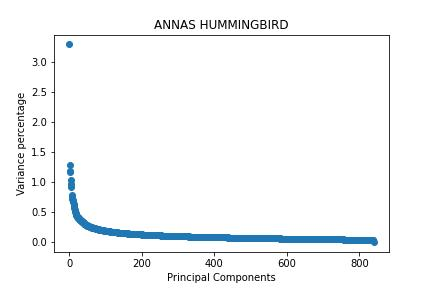
\includegraphics[width=0.35\textwidth]{plots/variance-ANN.jpg}
    }
    \subfloat[Flamingo]{
        \label{ref_labe4}
        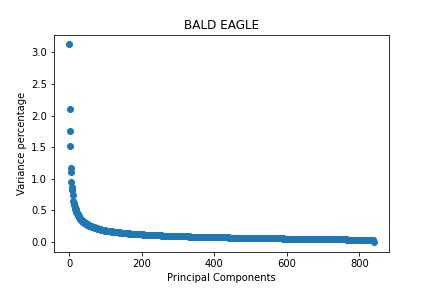
\includegraphics[width=0.35\textwidth]{plots/variance-BAL.jpg}
    } 
    \subfloat[Bald Eagle]{
        \label{ref_labe1}
        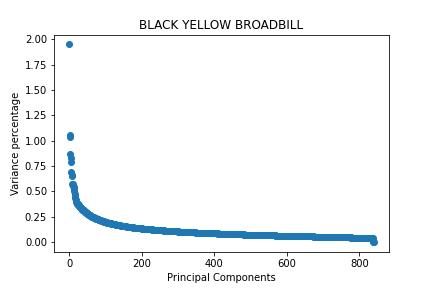
\includegraphics[width=0.35\textwidth]{plots/variance-BLA.jpg}
    }\\
    \subfloat[Annas Hummingbird]{
        \label{ref_labe2}
        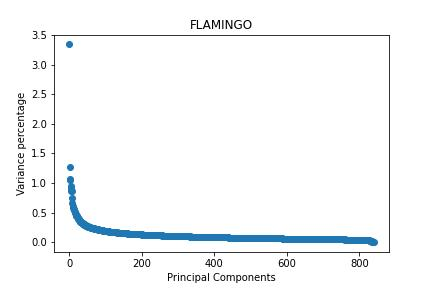
\includegraphics[width=0.4\textwidth]{plots/variance-FLA.jpg}
    }
    \subfloat[Scarlet Macaw]{
        \label{ref_labe3}
        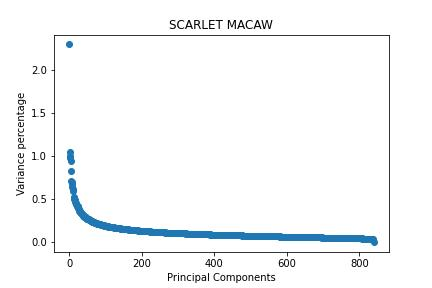
\includegraphics[width=0.4\textwidth]{plots/variance-SCA.jpg}
    }
    
    \caption{Variance explained by principal components.}
\end{figure} 

All 5 plots show a similar distribution of the explained variance per eigenbird for each species. In each graph the amount of variance seems to level off around the 180 - 200 mark, meaning that this range of values serve as a good cutoff to separate the most meaningful features for each bird. In this case a reasonable value for $K$ would be to select the first 180 components. Therefore, by implementing our approach using this value of $K$ and calculating the residuals for each test image, we can classify each sample simply by selecting the lowest value when compared to each species. The time it took for the model to train and run from image input to image classification was taking into account as a measure of model efficiency. It took 3475.41 seconds to complete or around 57.92 minutes. The following were the results: 

\begin{figure}[h]
    \centering
    
    \subfloat[Classification Metrics]{
        \label{ref_labe1}
        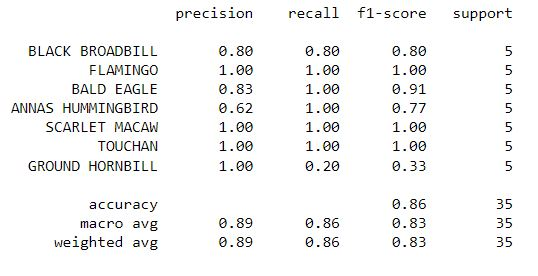
\includegraphics[width=0.6\textwidth]{plots/dim-red-results.jpg}
    } \\
    \subfloat[Confusion Matrix]{
        \label{ref_labe4}
        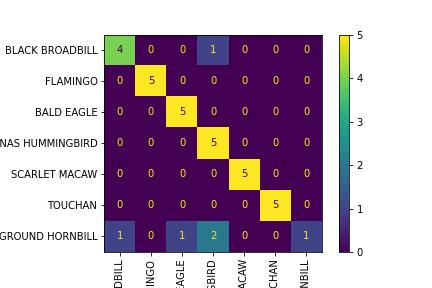
\includegraphics[width=0.6\textwidth]{plots/dim-red-cf.jpg}
    }
    \caption{Dimensionality Reduction Evaluation.}
\end{figure} 

A pretty decent result given the high number of labels and the low amount of training images. \\


\subsection{Density Estimation}

Density estimation is another method that can be used to build a bird classifier. This method is an unsupervised learning technique that is used to find where similar data clusters together due to having similar features. Clustering is a technique that takes advantage of density estimation through different dimensions for multivariate data. In this case, a non-parametric approach called Kmeans clustering will be used on our training images to find which ones are the most similar to each other, in effect creating $D$ clusters of images that based on the majority label inside the cluster each one, will be labeled as belonging to a specific type of bird. Using a new test image $y$, we can predict to which cluster is most likely to belong to and classify $y$ as the label assigned to the cluster. \\

The methodology itself consists of using the pre-processed data to build our training matrix $A$ where each row represents an image vector, and each column represents the pixel values of said vector for all the species. The entire matrix was then scaled by 255 to bound our data between 0 and 1. The training images were passed into our Kmeans algorithm which calulates $C$ cluster centroids randomly, and assigns the closes data points to each centroid. Each data point is then labeled based on which centroid is closest to. The centroids are then recalculated as the average of all the labeled data points in their respective cluster, and the process then repeats iteratively until there is no change. The dimensions for each data point will be the pixel values for each one of the pictures. The number of clusters will be selected by plotting the sum of all the square distances of each data point to their respective cluster centroid using different values for number of clusters. We do this because in theory the ideal number to use for the cluster parameter is the one that reduces the distance between each data point to their respective centroid without overfitting the data, this validation is popularly known as the elbow method. Figure 6 shows us the total sum of squares distances based on a range of 1 to 800 clusters used in our model. \\

\begin{figure}[h]
    \centering
    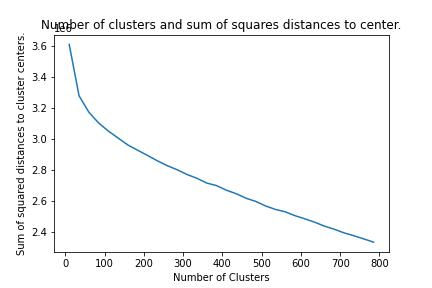
\includegraphics[width=0.7\textwidth]{plots/den-est-valid2.jpg}
    \caption{Total sum of squares distances to centroids.}
\end{figure}

Our plot does not seem to have a clear elbow where the number of clusters seems to have a big reduction on the distance to each centroid. This might mean that our algorithm is failling to capture the relationship between the images well. One possible reason might be due to our data having a non-linear relationship that kmeans can't account for. Another might be due to the curse of dimensionality; which explains that as the number of dimensions in our data increases, euclidian distance does not become a good metric to perform the separation of the data. Nonetheless, Let's select an arbitrary middle value in our plot and evaluate our test data to see the results. We perform our approach in order to classify our test data using Kmeans and a value of 150 for $C$. The model training and classification operation took aproximitely 622 seconds and gave the following result:\\

\begin{figure}[h]
    \centering
    
    \subfloat[Classification Metrics]{
        \label{ref_labe1}
        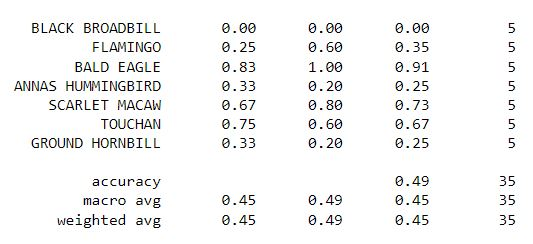
\includegraphics[width=0.6\textwidth]{plots/den-est-results.jpg}
    } \\
    \subfloat[Confusion Matrix]{
        \label{ref_labe4}
        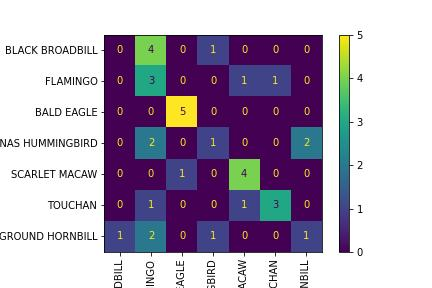
\includegraphics[width=0.6\textwidth]{plots/den-est-cf.jpg}
    }
    \caption{Density Estimation results.}
\end{figure} 

A much lower accuracy score compared to other approaches, some potential fixes to inrease this value might be to experiment with other clustering approaches that better capture the non-linear nature of the data or appling dimensionality reduction to curve the curse of dimensionality. \\


\subsection{Classification}
It is intuitive that some of the first approaches to try when making an image classifier would be to use some of the classic algorithms for supervised learning classification like SVM, Kernel SVM, K-nearest neighbors, logistics regression, and more. In this section we will implement the aforementioned approaches using our image data. Each bird classifier will be evaluated based on accuracy as well as being compared to all the others to decide which one is the best. K-nearest neighbors and kernel Support vector machines will serve as our non-linear classifiers, while linear SVM and logistic regression will try to capture the linear relationship between the data. All images will go through the same pre-processing steps as specified in the respective section in the methodology. Furthermore, our data will also be subjected to dimensionality reduction using principal component analysis due to the high number of pixel features that could cause overfitting when making our classifications. A kernelized implementation of PCA will also be performed in the data to try to capture the variance in the data in a non-linear subspace; it will then be evaluated on each supervised learning algorithm separately. The optimal parameters for each model will be found by performing 5 fold cross-validation with the data, and finally the best scoring combination of dimensionality reduction and classification model with optimal parameters will be evaluated in the test data. The highest scores of each model with it's optimal parameters from applying a grid search 5 fold cross-validation step are as follows: 

\begin{table}[h]
    \centering
    \begin{tabular}{ |M{2.5cm}|M{2cm}|M{2cm}|}
	 \hline
	 & PCA & KPCA \\
	 \hline
	 Model & Accuracy&Accuracy\\
	 \hline
	 K-NN & 0.36 &  0.46  \\
	 Logistic Re. & 0.51 & 0.53 \\
	 Linear SVM& 0.56 & 0.56 \\
	 Kernel SVM& 0.70 & 0.68 \\
	 \hline
   \end{tabular} \\
   \caption{Model evaluations}
\end{table}

Due to one fifth of our training data being used for validation purposes the scores might be lower than when the whole training data is used when building our best model to classify our test set. Out of all the models evaluated Kernel SVM proved to be the best when combined with a linear dimensionality reduction technique. This is due to the non-linear nature of this approach being able to capture the complexity of the different patterns present in each image better. KNN while non-linear, suffers from the curse of dimensionality as Kmeans did giving it a much lower accuracy score than the other methods. Logistic regression and linear SVM had very similar scores when trying to capture the linear relationship in the data. Using our best performing approach now we can evaluate or test data to get the following classification metrics:

\begin{figure}[h]
    \centering
    
    \subfloat[Classification Metrics]{
        \label{ref_labe1}
        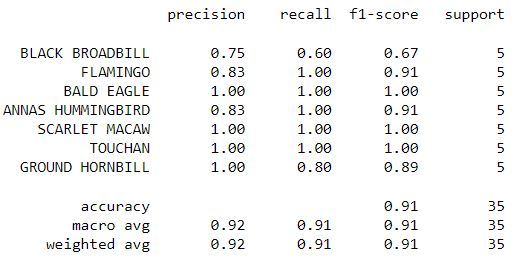
\includegraphics[width=0.55\textwidth]{plots/svm-results.jpg}
    } 
    \subfloat[Confusion Matrix]{
        \label{ref_labe4}
        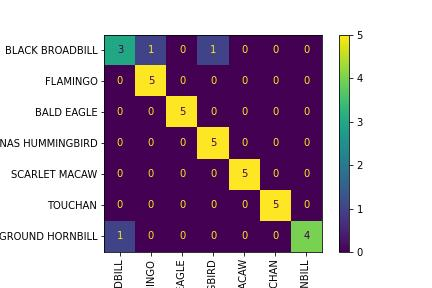
\includegraphics[width=0.6\textwidth]{plots/svm-cf.jpg}
    }
    \caption{$SVC\{C=4,kernel=rbf,gamma=scale,random\_state=2\}$}
\end{figure} 

 So far, kernel SVM has proven to be the best method to build our bird identifier. The time it took to train and predict ended up being 399 seconds; much faster than our second best performing approach as well. \\

\subsection{Deep Learning} 

Our final approach consists of diving into the field of deep learning for image classification. Deep learning is a subfield of machine learning that specializes on reproducing the way the human brain thinks to solve certain problems. It does this by using artificial neural networks; a mathematical representation of a composition of neurons signaling to each other. This field has proven to have an endless number of real life applications when it comes to using data to gain insight on an input. In this case, we will implement a variation of this approach called a convolutional neural network. This algorithm is specifically designed to deal with the high dimensionality that images present. It is important to note that for an 64x64x3 image the number of dimensions that each alogrithm has to take into account is 12,288, combined with more than 5,880 distinct training images we get more than 72,000,000 distinct values that need to be taken into account. Performing the necessary computations to learn from the data becomes a tedious and long task to do in a normal computer. CNNs solve this issue by taking advantage of two ideas: Convolutions and subsampling. Convolution is the process of extracting the high level features of an image through the use of a filter, for each feature we perform subsampling to reduce the spatial size of the convolution to reduce the computational power necessary for the algorithm to work. We alternate between this two methods in the form of layers until we come out with an output that has been trained to understand the features of each species. this output will be flattened into a vector and fed into a dense traditional feed forward neural network to make our classification. Due to this small amount of training images we might have a tendency to overfit to our training data and fail to generalize properly when validating our model. To prevent this, some neurons will be turn off randomly during the training process to prevent the network becoming too dependent in the data. This concept is known as dropout and is used as a regularization technique when using CNNs. \\

For this approach the training data was reshaped into a 4 dimensional matrix of shape Mx64x64x3 to serve as an input to our network. One-hot encoding was performed to each of our training labels as well to transform it into a 1 dimensional vector which combined between all the training images gives us a matrix of size MxK, where each row represents the label vector of each training image and each column the species that it belongs to. For our network, The implementation was done using the Keras library to build our network sequentially; each layer consisted of a convolution step, a leaky relu activation function to capture non-linear relationships, and a max pooling step that serves as our subsampling for that layer. Dropout was implemented aswell after each layer to prevent overfitting and finally a dense layer was added to input our flatten data and make our classification. The summary of the network can be seen below (figure 9): 

\pagebreak

\begin{figure}[h]
    \centering
    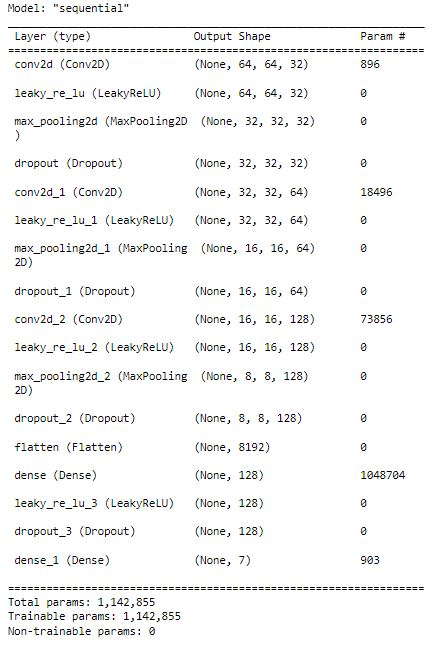
\includegraphics[width=0.68\textwidth]{plots/CNN-structure.jpg}
    \caption{CNN Architecture.}
\end{figure} 

\bigskip
\bigskip

A batch size of 64 was specified and the network was set up to run for 20 epochs for training purposes. The network was set up to calculate accuracy as well as loss of the network on both the validation set and the training data at each epoch. The results of this process was saved and plotted against the number of epochs to visualize the learning process as well as to check for overfitting in our model. Figure 10 shows the result of the previous step: \\

\pagebreak

\begin{figure}[h]
    \centering
    
    \subfloat[Classification Metrics]{
        \label{ref_labe1}
        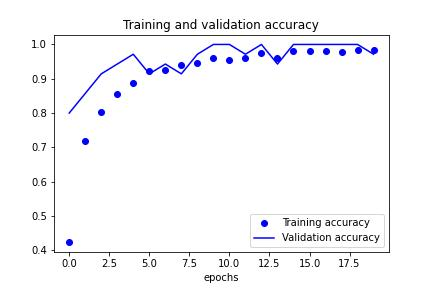
\includegraphics[width=0.5\textwidth]{plots/cnn-accuracy.jpg}
    }
    \subfloat[Confusion Matrix]{
        \label{ref_labe4}
        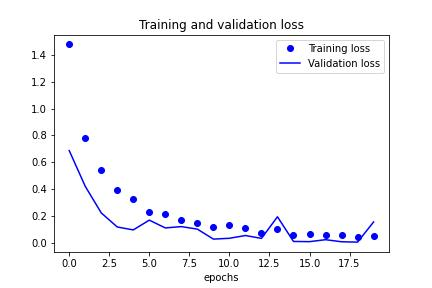
\includegraphics[width=0.5\textwidth]{plots/cnn-loss.jpg}
    }
    \caption{CNN validation by epoch}
\end{figure} 

These plots shows us good performance and little overfitting. Using our trained network we can now evaluate our test data and see the results in figure 11: 

\begin{figure}[h]
    \centering
    
    \subfloat[Classification Metrics]{
        \label{ref_labe1}
        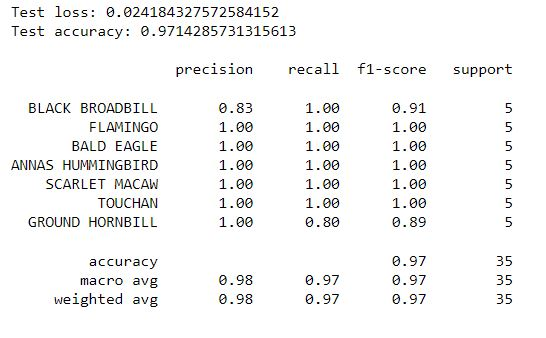
\includegraphics[width=0.55\textwidth]{plots/CNN-results.jpg}
    }
    \subfloat[Confusion Matrix]{
        \label{ref_labe4}
        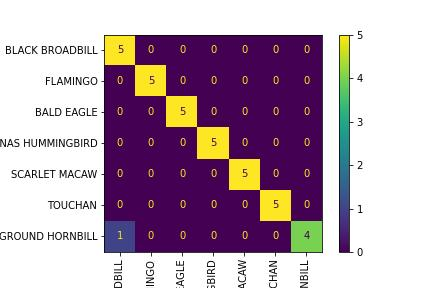
\includegraphics[width=0.6\textwidth]{plots/deep-learn-cf.jpg}
    }
    \caption{CNN results on test data.}
\end{figure}

This implemation took 675 seconds to train and make our prediction. While loger than our next best approach, this method proved to be the most accurate when building our bird classifier between all the different methods presented in our experiments. Even with the lack of training data this approach was able to generalize extremely well when presented with a new test set independent of our training samples. \\

\section{Evaluation and Final Results}

Out of all approaches presented the results of the most optimal technique in each category can be summarized in the following table:

\begin{table}[h]
    \centering
    \begin{tabular}{ |M{2.5cm}|M{2cm}|M{2cm}|}
	 \hline
	 Model & Accuracy&Time(s)\\
	 \hline
	 Eigenbirds & 0.86 &  3475.41  \\
	 Kmeans & 0.54 & 622 \\
	 PCA/KSVM & 0.91 & 399 \\
	 CNN & 0.97 & 675 \\
	 \hline
   \end{tabular} \\
   \caption{Overrall results.}
\end{table}

The time column is in seconds and it encompasses both training time and performing the classification on the testing set. Convolutional neural networks proved to be the most accurate approach and the best one in capturing the complex differences of different pictures of species of birds. PCA combined with a kernel SVM proved to be the fastest by almost half, becoming a good second option to perform in case efficiency is the priority when building the classifier. \\



Using our most optimal model we can now use it on a bigger set of data in order to identify as many species as possible. We will use a CNN in order to classify between 30 different species of birds for our final test. The model will be trained using the same methodology applied on the prototyping stage. Data augmentation will be used in the data in order to increase our training samples to be around 1080 pictures per species, the amount of pictures used for validation and testing will remain the same as in the prototyping stage. Using our new data we can train, validate, and test our model to get the results shown in figure 12 and 13. A picture example of each of the 30 species used can be seen on appendix A. Even though we increased the number of species to 30, the model still performed extremely well with an accuracy of 93\%. \\

This implementation proved to be robust even with the small sample of training data used to build our model. The time for training and classification increased only by around 3000 seconds or 50 minutes, but given the scope of the data this could be considered an acceptable efficiency. Further applications and scalibility could be applied to this method as well. More species could be added and other data augmentation techniques could be used in order to compensate with the low amount of samples for our training images. A real time video classifier could also be implemented by checking frame by frame and classifying the birds present in the video using our model. \\ \\

A more specific look into the classification matrix of our model can be seen below:

\begin{figure}[p]
    \centering
    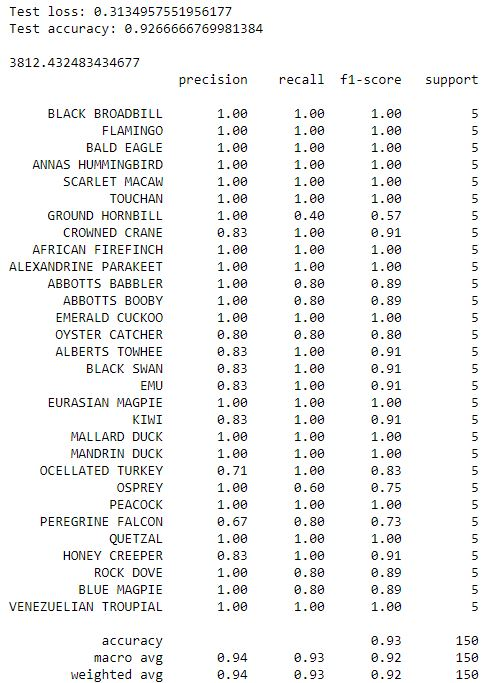
\includegraphics[width=0.7\textwidth]{plots/CNN-results_final.jpg}
    \caption{CNN results on test data.}
\end{figure}


\begin{figure}[p]
    \centering
    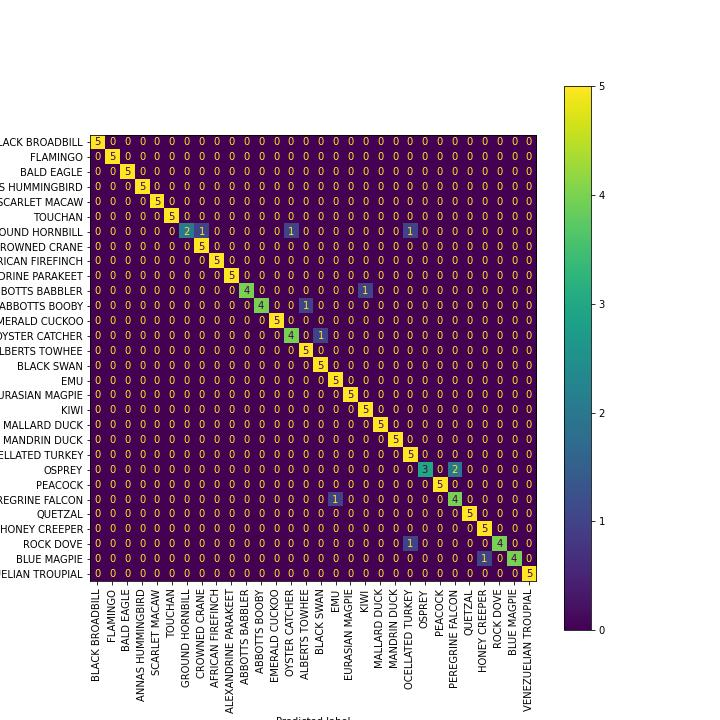
\includegraphics[width=1\textwidth]{plots/deep-learn-cf_final.jpg}
    \caption{CNN results on test data.}
\end{figure}

\pagebreak

In conclusion there exists many different approaches that can be implemented for image classification, it is a matter of finding the right combinations of tools and methodologies to accomplish the specific task that best would solve your problem. In this case we were able to build a quick and efficient bird species identifier implementing several distinct ideas that provided us with a range of different results, some better than others. Overrall the exploration of all this methodologies does a good job of proving there are many roads that could lead to your desired destination, it is only a matter of finding the one that fits the best.


\begin{appendices}
\section{30 Evaluated Species}
\begin{figure}[h]
    \centering
    
    \subfloat[Black Broadbill]{
        \label{ref_lael1}
        \includegraphics[width=0.2\textwidth]{data/birds/train/1BLACK YELLOW BROADBILL/001.JPG}
    }
    \subfloat[Flamingo]{
        \label{ref_lbel4}
        \includegraphics[width=0.2\textwidth]{data/birds/train/2FLAMINGO/011.JPG}
    } 
    \subfloat[Bald Eagle]{
        \label{ref_label1}
        \includegraphics[width=0.2\textwidth]{data/birds/train/3BALD EAGLE/019.JPG}
    }
    \subfloat[Annas Hummingbird]{
        \label{ref_label2}
        \includegraphics[width=0.2\textwidth]{data/birds/train/4ANNAS HUMMINGBIRD/006.JPG}
    }
    \subfloat[Scarlet Macaw]{
        \label{ref_label3}
        \includegraphics[width=0.2\textwidth]{data/birds/train/5SCARLET MACAW/016.JPG}
    }\\
    \subfloat[Ground Hornbill]{
        \label{ref_label3}
        \includegraphics[width=0.2\textwidth]{data/birds/train/9ABYSSINIAN GROUND HORNBILL/007.JPG}
    }
     \subfloat[Touchan]{
        \label{ref_label4}
        \includegraphics[width=0.2\textwidth]{data/birds/train/6TOUCHAN/013.JPG}
    }
    \subfloat[Crowned Crane]{
        \label{ref_lael1}
        \includegraphics[width=0.2\textwidth]{data/birds/train/AAFRICAN CROWNED CRANE/017.JPG}
    }
    \subfloat[Firefinch]{
        \label{ref_lbel4}
        \includegraphics[width=0.2\textwidth]{data/birds/train/AAFRICAN FIREFINCH/006.JPG}
    } 
    \subfloat[Alexandrine parakeet]{
        \label{ref_label1}
        \includegraphics[width=0.2\textwidth]{data/birds/train/AALEXANDRINE PARAKEET/017.JPG}
    } \\
    \subfloat[Abbotts Babler]{
        \label{ref_label2}
        \includegraphics[width=0.2\textwidth]{data/birds/train/BABBOTTS BABBLER/013.JPG}
    }
    \subfloat[Abbotts Booby]{
        \label{ref_label3}
        \includegraphics[width=0.2\textwidth]{data/birds/train/BABBOTTS BOOBY/002.JPG}
    }
    \subfloat[Emerald Cuckoo]{
        \label{ref_lael1}
        \includegraphics[width=0.2\textwidth]{data/birds/train/BAFRICAN EMERALD CUCKOO/053.JPG}
    }
    \subfloat[Oyster Catcher]{
        \label{ref_lbel4}
        \includegraphics[width=0.2\textwidth]{data/birds/train/BAFRICAN OYSTER CATCHER/009.JPG}
    } 
    \subfloat[Alberts Towhee]{
        \label{ref_label1}
        \includegraphics[width=0.2\textwidth]{data/birds/train/BALBERTS TOWHEE/016.JPG}
    } \\
    
     \caption{Selected Species part 1}
    \label{selected species}
\end{figure}


\begin{figure}[h]
    \centering
    
    \subfloat[Black Swan]{
        \label{ref_label2}
        \includegraphics[width=0.2\textwidth]{data/birds/train/BBLACK SWAN/011.JPG}
    }
    \subfloat[Emu]{
        \label{ref_label3}
        \includegraphics[width=0.2\textwidth]{data/birds/train/BEMU/012.JPG}
    }
    \subfloat[Magpie]{
        \label{ref_lael1}
        \includegraphics[width=0.2\textwidth]{data/birds/train/BEURASIAN MAGPIE/016.JPG}
    }
    \subfloat[Kiwi]{
        \label{ref_lbel4}
        \includegraphics[width=0.2\textwidth]{data/birds/train/BKIWI/061.JPG}
    } 
    \subfloat[Mallard Duck]{
        \label{ref_label1}
        \includegraphics[width=0.2\textwidth]{data/birds/train/BMALLARD DUCK/001.JPG}
    } \\
    \subfloat[Mandrin Duck]{
        \label{ref_label2}
        \includegraphics[width=0.2\textwidth]{data/birds/train/BMANDRIN DUCK/001.JPG}
    }
    \subfloat[Ocellated Turkey]{
        \label{ref_label3}
        \includegraphics[width=0.2\textwidth]{data/birds/train/BOCELLATED TURKEY/001.JPG}
    }
    \subfloat[Osprey]{
        \label{ref_lael1}
        \includegraphics[width=0.2\textwidth]{data/birds/train/BOSPREY/001.JPG}
    }
    \subfloat[Peacock]{
        \label{ref_lbel4}
        \includegraphics[width=0.2\textwidth]{data/birds/train/BPEACOCK/007.JPG}
    } 
    \subfloat[Falcon]{
        \label{ref_label1}
        \includegraphics[width=0.2\textwidth]{data/birds/train/BPEREGRINE FALCON/019.JPG}
    } \\
    \subfloat[Quetzal]{
        \label{ref_label2}
        \includegraphics[width=0.2\textwidth]{data/birds/train/BQUETZAL/014.JPG}
    }
    \subfloat[Honey Creeper]{
        \label{ref_label3}
        \includegraphics[width=0.2\textwidth]{data/birds/train/BRED HONEY CREEPER/001.JPG}
    }
    \subfloat[Dove]{
        \label{ref_lael1}
        \includegraphics[width=0.2\textwidth]{data/birds/train/BROCK DOVE/013.JPG}
    }
    \subfloat[Blue Magpie]{
        \label{ref_lbel4}
        \includegraphics[width=0.2\textwidth]{data/birds/train/BSRI LANKA BLUE MAGPIE/030.JPG}
    } 
    \subfloat[Troupial]{
        \label{ref_label1}
        \includegraphics[width=0.2\textwidth]{data/birds/train/BVENEZUELIAN TROUPIAL/019.JPG}
    } \\
  
    \caption{Selected Species part 2}
    \label{selected species}
    
\end{figure}
\end{appendices}
\end{singlespace}
\end{document}
